% Zurich Tree Management — Research paper
% Vision-oriented study; figures in figures/

\documentclass[12pt,a4paper]{article}
\usepackage[utf8]{inputenc}
\usepackage[T1]{fontenc}
\usepackage{lmodern}
\usepackage{geometry}
\usepackage{hyperref}
\usepackage{url}
\usepackage{booktabs}
\usepackage{parskip}
\usepackage{enumitem}
\usepackage{graphicx}
\usepackage{amsmath}
\usepackage{longtable}
\usepackage{array}
\usepackage{tikz}
\usetikzlibrary{arrows.meta,positioning,fit,backgrounds}

\geometry{margin=2.5cm}
\linespread{1.12}
\hypersetup{colorlinks=true,urlcolor=blue,citecolor=blue}
\graphicspath{{figures/}}

\newcommand{\appname}{Zurich Tree Management Application}
\newcommand{\maybeincludegraphics}[2][]{%
  \IfFileExists{figures/#2}{%
    \includegraphics[#1]{#2}%
  }{%
    \fbox{\parbox[c][0.22\textheight][c]{0.92\linewidth}{\centering\small\textit{Place screenshot: \texttt{#2}}}}}%
}

\title{Situated Civic Infrastructure on the Map:\\
       A Design-Research Vision for Service-Request--Centred Urban Tree Governance}
\author{Suad Arzimanli \\ \texttt{suad.arzimanli@gmail.com}}
\date{}

\begin{document}
\maketitle

\begin{abstract}
Urban trees are simultaneously ecological assets, safety-critical infrastructure, and sites of everyday citizen concern. Yet municipal responses to tree-related service requests remain fragmented across map interfaces, case-management systems, and tacit field knowledge. This paper presents a \textbf{design-research vision} embodied in the \appname{}: a geospatial demonstrator that treats the \textbf{service request (SR) as the narrative and organisational anchor} through which open government data, inspection logic, work-order execution, and activity planning are made mutually intelligible to citizens and arborists alike.

Rather than reporting implementation detail as an end in itself, the paper asks what such a system \textbf{represents} for the future of public green-infrastructure governance: a shift from map-as-display toward \textbf{map-as-venue for accountable workflow}; from siloed records toward \textbf{phase-aware, bilingual civic operations}; and from proprietary enterprise stacks toward \textbf{composable public-data architectures} that municipalities can study, critique, and adapt. Drawing on design science, sociotechnical systems theory, and open-government scholarship, we articulate research questions, a conceptual model of SR-centred phases, and implications for equity, institutional trust, and climate-resilience planning.

The runnable artifact---integrating the City of Zürich \emph{Baumkataster} with structured inspection and work-order lifecycles---functions as a \textbf{research instrument}: a material argument that operational software should be legible, ethically bounded, and aligned with how frontline staff actually speak about cases. We conclude with a programme for further research spanning participatory design with forestry departments, cross-city comparative governance, and longitudinal studies of how digital intake reshapes citizen--state relations around urban nature.

\medskip
\noindent\textbf{Disclaimer:} The \appname{} is an \textbf{independent research demonstrator}. It is not affiliated with, endorsed by, or operated on behalf of the City of Zürich or any municipal agency.
\end{abstract}

\noindent\textbf{Keywords:} urban forestry governance; service-request workflow; open government data; sociotechnical design; geospatial civic infrastructure; digital public services; design science; accountable automation; climate adaptation; bilingual administration.

\tableofcontents
\listoffigures
\newpage

%======================================================================
\section{Introduction: Why urban trees need a new digital contract}
\label{sec:intro}

\subsection{The problem of invisible infrastructure}

Street and park trees form what urban scholars have described as \textbf{living infrastructure}: they moderate heat, manage stormwater, support biodiversity, and shape the experiential quality of neighbourhoods \cite{beatley2011,escobedo2011}. Unlike pipes or power lines, however, trees are \textbf{highly visible and emotionally salient} to residents. A broken branch, an obstructed sidewalk, or a desired planting triggers contact with the municipality---not as an abstract ``ticket,'' but as a claim on shared public space.

Municipal forestry units therefore operate at a distinctive intersection: they are \textbf{ecological stewards}, \textbf{safety regulators}, and \textbf{frontline service providers}. Digital systems intended to support them often fail this hybrid mission. Maps show \emph{where} trees are; enterprise resource planning shows \emph{what} was billed; customer-relationship modules show \emph{who} called. Rarely does a single interface sustain the \textbf{end-to-end narrative} from citizen intent through inspection, work order, and documented closure---while remaining geographically grounded.

\subsection{Research gap}

Geographic information systems (GIS) research has matured techniques for spatial analysis and web mapping \cite{goodchild2007}. Parallel streams in e-government examine open data portals and transparency \cite{janssen2012}. Workflow and business-process management literatures formalise state machines and service orchestration \cite{recker2016}. What remains under-theorised in much of the existing literature is the \textbf{integrative design knowledge} that links:

\begin{enumerate}[label=(\roman*)]
    \item authoritative \textbf{open geospatial assets} (e.g.\ municipal tree cadastres);
    \item \textbf{case-centric operational memory} (inspections, work orders, assignments);
    \item \textbf{human accountability norms} (comments, signatures, closure categories);
    \item \textbf{multilingual and multicultural public service} in global cities.
\end{enumerate}

This gap is not merely technical. It is \textbf{epistemic}: organisations lack shared conceptual language for what a ``case'' \emph{is} when the object of concern is both a biological entity and a civic request.

\subsection{Research questions}

This study is guided by the following questions:

\begin{description}
    \item[RQ1] \textbf{Anchoring.} How does treating the service request as the primary organisational unit reshape the intelligibility of urban tree workflows for operators and researchers?
    \item[RQ2] \textbf{Situatedness.} In what ways does map-integrated intake change the \emph{situated} character of civic infrastructure work---binding location, species context, and procedural state?
    \item[RQ3] \textbf{Openness.} What governance possibilities and risks arise when operational demonstrators compose public OGD layers with locally controlled case records?
    \item[RQ4] \textbf{Vision.} What future municipal capabilities---equity analytics, resilience planning, participatory budgeting---does such an architecture \emph{prefigure}, even when not yet implemented?
\end{description}

\subsection{Contribution}

The contribution is threefold:

\begin{enumerate}[label=\textbf{C\arabic*:}]
    \item A \textbf{conceptual model} of SR-centred phased workflow for urban forestry (\S\ref{sec:model}), offered as transferable design knowledge rather than a single-vendor specification.
    \item A \textbf{design-research artifact} (\S\ref{sec:artifact}) that materialises the model using Zürich OGD \emph{Baumkataster} data, documented through figures suitable for scholarly dissemination.
    \item A \textbf{normative vision} (\S\ref{sec:vision}) of next-generation civic green-infrastructure platforms, with explicit ethical boundaries and a future research agenda (\S\ref{sec:conclusion}).
\end{enumerate}

\subsection{Structure}

Section~\ref{sec:theory} situates the work theoretically. Section~\ref{sec:model} presents the conceptual model. Section~\ref{sec:method} describes design-research methodology. Section~\ref{sec:artifact} introduces the artifact as research instrument with figures. Section~\ref{sec:vision} develops the forward-looking vision. Section~\ref{sec:discussion} discusses implications; Section~\ref{sec:limits} limitations and ethics; Section~\ref{sec:conclusion} concludes.

%======================================================================
\section{Theoretical framing}
\label{sec:theory}

\subsection{Sociotechnical systems and the morality of workflows}

Classic sociotechnical systems theory insists that work organisation and technology co-evolve \cite{trist1981}. In municipal forestry, workflow is not a neutral diagram: deciding that an inspection may close as ``no work'' versus ``resolution'' is a \textbf{moral and budgetary act}---it allocates scarce crew time, determines liability narratives, and closes or opens citizen expectations.

This work argues that such software must be analysed not only for usability but for \textbf{how it distributes agency}. Who may create a case? Who must comment before closure? Who sees internal notes versus public-facing status? The \appname{} encodes such choices explicitly, making them available for critique---a property aligned with \emph{reflective design} traditions in human--computer interaction \cite{sengers2005}.

\subsection{Open government data as civic infrastructure}

Open Government Data (OGD) initiatives position spatial datasets as \textbf{public infrastructure} rather than departmental by-products \cite{janssen2012}. The Zürich \emph{Baumkataster} exemplifies a trend toward machine-readable urban nature inventories. Yet OGD alone does not constitute service delivery: citizens still experience \textbf{procedural opacity} if intake channels are decoupled from the same geographic truth.

We argue that further research should examine \textbf{compositional architectures}: public layers (trees, boundaries, hazards) interleaved with institutionally governed layers (cases, assignments, audit). Such composition respects democratic transparency for \emph{what exists in the city} while preserving legitimate confidentiality for \emph{who reported what}.

\subsection{Digital twins, living systems, and modesty of claim}

Smart-city discourse often invokes ``digital twins''---real-time mirror worlds for simulation and control \cite{batty2018}. Urban trees resist naive twinning: they grow, die, are pruned, and are contested politically. A more honest research stance adopts \textbf{modest digital representation}: maps and records that are \textbf{actionable and accountable} rather than exhaustively predictive.

The \appname{} represents this modesty. It does not forecast canopy carbon sequestration or optimise fleet routing at city scale. Instead, it demonstrates how \textbf{faithful workflow memory} attached to geographic objects supports the incremental, case-by-case reasoning through which forestry departments actually survive peak complaint seasons.

\subsection{Public service language and bilingual administration}

In linguistically diverse municipalities, interface language is governance. Bilingual English--German support in the demonstrator is not cosmetic: it signals that \textbf{operational categories} (request types, phases, closure reasons) must be negotiable across clerical, field, and citizen literacies. Research in public administration increasingly recognises multilingual UX as \textbf{equity infrastructure} \cite{rubio2019}.

%======================================================================
\section{A conceptual model: service-request--centred phases}
\label{sec:model}

\subsection{The SR as epistemic anchor}

We propose that the \textbf{service request} should function as the \textbf{epistemic anchor}---the unit to which utterances, statuses, and geographic references attach. Inspections and work orders are not parallel ``modules'' in separate mental models; they are \textbf{phases of the same civic story}.

This anchoring responds to RQ1. When operators search ``SR\,10005'' rather than an inspection identifier, they reproduce organisational memory. Software that mirrors this practice reduces \textbf{cognitive translation cost} between map, desk, and oral handover.

\subsection{Phase ontology}

Operational \emph{phase} is derived from the joint state of SR, inspection, and work-order entities (Table~\ref{tab:phase}). Phases are \textbf{legible abstractions} for filtering and public communication, not replacements for legal record-keeping.

\begin{table}[htbp]
\centering
\caption{Phase ontology for urban tree service requests (conceptual).}
\label{tab:phase}
\begin{tabular}{@{}p{0.22\linewidth}p{0.68\linewidth}@{}}
\toprule
\textbf{Phase} & \textbf{Meaning for citizens and staff} \\
\midrule
Service request & Intake recorded; geographic and contact context captured; inspection may await action. \\
Inspection & Site assessment in progress; findings may lead to closure without works or to scheduled intervention. \\
Work order & Field execution authorised; contractor or crew assignment; safety and traffic measures may apply. \\
Closed & Case resolved; documented outcome (e.g.\ no work, completed works, information provided). \\
\bottomrule
\end{tabular}
\end{table}

\subsection{Conceptual architecture}

Figure~\ref{fig:vision-model} presents the integrative architecture at the level of \textbf{ideas}, independent of any single framework or vendor.

\begin{figure}[htbp]
\centering
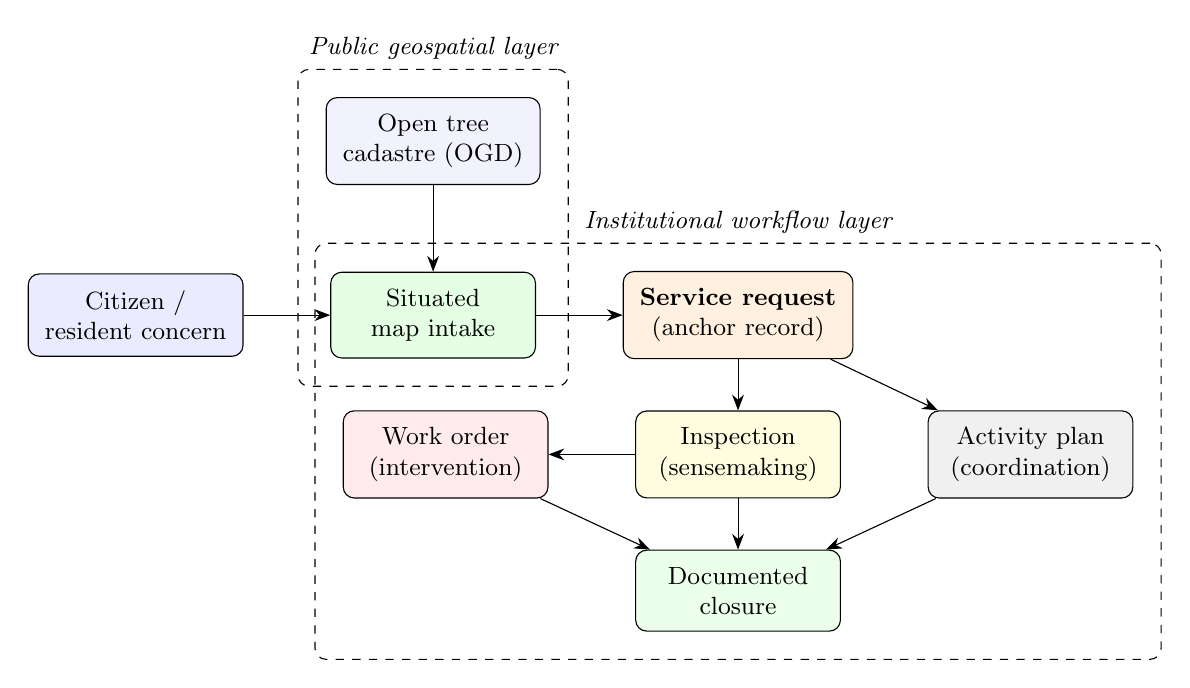
\begin{tikzpicture}[
    node distance=0.65cm and 1.1cm,
    box/.style={draw, rounded corners, align=center, font=\small, inner sep=6pt, minimum width=2.6cm},
    layer/.style={draw, dashed, inner sep=10pt, rounded corners}
]
\node[box, fill=blue!8] (citizen) {Citizen /\\resident concern};
\node[box, fill=green!10, right=of citizen] (map) {Situated\\map intake};
\node[box, fill=orange!12, right=of map] (sr) {\textbf{Service request}\\(anchor record)};
\node[box, fill=yellow!12, below=of sr] (insp) {Inspection\\(sensemaking)};
\node[box, fill=red!8, left=of insp] (wo) {Work order\\(intervention)};
\node[box, fill=gray!12, right=of insp] (act) {Activity plan\\(coordination)};
\node[box, fill=green!8, below=of insp] (closed) {Documented\\closure};

\node[box, fill=blue!5, above=1.1cm of map] (ogd) {Open tree\\cadastre (OGD)};

\draw[-{Stealth[length=2mm]}] (citizen) -- (map);
\draw[-{Stealth[length=2mm]}] (map) -- (sr);
\draw[-{Stealth[length=2mm]}] (ogd) -- (map);
\draw[-{Stealth[length=2mm]}] (sr) -- (insp);
\draw[-{Stealth[length=2mm]}] (insp) -- (wo);
\draw[-{Stealth[length=2mm]}] (insp) -- (closed);
\draw[-{Stealth[length=2mm]}] (wo) -- (closed);
\draw[-{Stealth[length=2mm]}] (sr) -- (act);
\draw[-{Stealth[length=2mm]}] (act) -- (closed);

\begin{scope}[on background layer]
\node[layer, fit=(map)(ogd), label={[font=\small\itshape]above:Public geospatial layer}] {};
\node[layer, fit=(sr)(insp)(wo)(act)(closed), label={[font=\small\itshape]above:Institutional workflow layer}] {};
\end{scope}
\end{tikzpicture}
\caption{Conceptual model: the service request anchors situated map intake (fed by open tree data) to inspection, optional work order, coordinated activities, and accountable closure.}
\label{fig:vision-model}
\end{figure}

\subsection{Dual surfaces: map and desk}

RQ2 emphasises \emph{situatedness}. The model deliberately provides \textbf{two coupled surfaces}:

\begin{itemize}
    \item \textbf{Map surface} --- maintains geographic situational awareness; supports discovery, spatial filtering, and ``what is near this tree?''
    \item \textbf{Desk surface} --- supports high-density case work; search, batch triage, and multi-tab editing without losing SR context.
\end{itemize}

Neither surface is subordinate. Further analysis should ask when clerical labour migrates between them, and whether mobile futures collapse the distinction---a question the demonstrator opens but does not settle.

%======================================================================
\section{Design-research methodology}
\label{sec:method}

\subsection{Design science in interpretive mode}

We adopt design science research (DSR) as articulated by Hevner et al.\ \cite{hevner2004}: knowledge through building. Here, DSR is paired with \textbf{interpretive depth}---the artifact is not only evaluated for utility but \textbf{read as a text} about municipal futures \cite{goldkuhl2019}.

Evaluation in this paper is \textbf{argumentative and demonstrative} rather than statistical:

\begin{itemize}
    \item \textbf{Coherence} --- Can phases, map symbology, and desk language be explained without contradiction?
    \item \textbf{Fidelity to practice} --- Do closure rules (comments, dates, typed resolutions) resemble forestry norms?
    \item \textbf{Transparency} --- Can governance choices be inspected and debated?
    \item \textbf{Transferability} --- Can other cities map their OGD assets and categories onto the model?
\end{itemize}

Formal user studies with operator $N$ and controlled task times are \textbf{deferred} to follow-on empirical work; this paper establishes the conceptual and visual foundation.

\subsection{Site selection: why Zürich as a research setting}

Zürich offers a pedagogically rich \textbf{research site}: a city with published tree cadastre data, internationally visible open-data culture, and forestry categories recognisable across European municipalities. Using Zürich OGD does not claim municipal partnership; it claims \textbf{realism of public data conditions}---latency, attribution, scale-dependent interaction---that synthetic maps cannot reproduce.

\subsection{Ethical stance of the demonstrator}

The artifact runs with \textbf{demo authentication} and local persistence to keep human subjects and operational systems out of scope. This is an ethical choice enabling classroom and academic review without exposing resident PII from live systems.

%======================================================================
\section{The artifact as research instrument}
\label{sec:artifact}

\subsection{What the application is---and is not}

The \appname{} is a \textbf{material hypothesis}: if you anchor workflow on the SR, integrate OGD trees at intake, and mirror phases on map and desk, operators can reason about cases with less fragmentation. It is \textbf{not} a procurement-ready product, a digital twin, or an official channel of the City of Zürich.

Figures~\ref{fig:map}--\ref{fig:activities} document the hypothesis visually. Replace placeholder boxes by adding PNG files to the \texttt{figures/} folder (see \texttt{figures/README.md}).

\subsection{Situated map interface}

\begin{figure}[htbp]
\centering
\maybeincludegraphics[width=\linewidth]{fig-map-overview.png}
\caption{Map surface: urban tree canopy from open cadastre data, phase-coded service-request markers, and spatial filtering. The map is the citizen-facing \emph{venue} where geographic truth and case geography meet.}
\label{fig:map}
\end{figure}

\begin{figure}[htbp]
\centering
\maybeincludegraphics[width=\linewidth]{fig-map-pick.png}
\caption{High-zoom interaction: selecting trees or nearby service requests within a walkable radius. Zoom gating teaches that \textbf{scale discipline}---when the city is visible versus when individual trees are actionable---is a design variable with equity implications (dense versus peripheral neighbourhoods).}
\label{fig:map-pick}
\end{figure}

\subsection{Service-request desk as organisational memory}

\begin{figure}[htbp]
\centering
\maybeincludegraphics[width=\linewidth]{fig-desk-queue.png}
\caption{Desk surface: searchable card queue organised by workflow phase. The desk externalises \textbf{organisational memory}---what is waiting, what is urgent, what step each SR occupies.}
\label{fig:desk-queue}
\end{figure}

\begin{figure}[htbp]
\centering
\maybeincludegraphics[width=\linewidth]{fig-desk-detail.png}
\caption{SR-centric detail: tabs for overview, administrative fields, inspection, work order, and activities under one case identifier. The layout embodies the epistemic anchor principle (RQ1).}
\label{fig:desk-detail}
\end{figure}

\subsection{Accountable transitions}

\begin{figure}[htbp]
\centering
\maybeincludegraphics[width=\linewidth]{fig-workflow-inspection.png}
\caption{Inspection transition: structured fields and mandatory commentary for closure categories. The form encodes \textbf{accountability norms}---decisions must be narrated, not merely clicked.}
\label{fig:workflow-inspection}
\end{figure}

\begin{figure}[htbp]
\centering
\maybeincludegraphics[width=\linewidth]{fig-activities.png}
\caption{Activity plan progress: category-specific coordination steps spawned with the SR. This prefigures \textbf{cross-departmental orchestration} without claiming full enterprise integration.}
\label{fig:activities}
\end{figure}

\subsection{Minimal technical reference}

Readers requiring implementation traceability may consult the project repository README and appendix (\S\ref{app:trace}). The central argument here rests on \textbf{what the screens mean}, not on framework versions.

%======================================================================
\section{Research vision: what this work prefigures}
\label{sec:vision}

\subsection{From reactive complaints to anticipatory green governance}

Today's forestry departments are largely \textbf{reactive}: storms and citizen calls drive schedules. SR-centred systems that bind geographic assets to closure histories accumulate \textbf{longitudinal memory}. Future research can ask whether such memory enables:

\begin{itemize}
    \item hotspot detection for repeat failures (species, age class, contractor);
    \item equity audits of response latency by neighbourhood;
    \item coupling with heat-island and canopy-cover plans under climate stress \cite{mcpherson2022}.
\end{itemize}

The demonstrator does not implement analytics; it \textbf{prepares the epistemic preconditions}---stable case IDs, phased states, georeferenced trees---without which analytics remain spreadsheet folklore.

\subsection{Participatory and deliberative extensions}

A visionary municipal platform might expose \textbf{sanitised case status} to residents (``your planting request is scheduled for inspection'') while preserving staff-only fields. Further research could integrate participatory budgeting for street trees \cite{sintomer2010} or deliberative forums on species selection---always with attention to digital divide and language access.

\subsection{Composable municipal stacks versus vendor lock-in}

Enterprise suites offer integration at the cost of \textbf{interpretive closure}: cities struggle to explain to councils how workflows map to citizen experience. Composable stacks---OGD layers, open APIs, inspectable case stores---support \textbf{democratic auditability}. RQ3 invites critical questions: who maintains proxies when OGD endpoints change? Who funds bilingual UX? Who owns case data at contract termination?

\subsection{Human--algorithm partnering without hype}

Unlike domains rushing toward opaque prediction, urban forestry benefits from \textbf{slower automation}: recommending inspection priority from drought stress models should remain explainable and overridable. The SR-centred model reserves a place for human sign-off at every transition---a design stance compatible with responsible AI principles \cite{floridi2019} without mandating machine-learning components.

%======================================================================
\section{Discussion}
\label{sec:discussion}

\subsection{Answering the research questions}

\textbf{RQ1 (Anchoring).} Treating the SR as anchor aligns digital navigation with oral culture of case handover. Risk: anchor fixation may obscure multi-tree incidents (block-level storm damage). Future models may need \textbf{parent incidents} linking several SRs---an extension the current artifact hints at via map-radius picking but does not formalise.

\textbf{RQ2 (Situatedness).} Map-integrated intake reduces ambiguous addresses and supports tree mis-identification checks against cadastre attributes. Situatedness also introduces \textbf{zoom inequality}: users who never reach actionable scale may experience the city as ``unclickable.'' Field studies should observe how training and device access mediate this inequality.

\textbf{RQ3 (Openness).} Composing OGD with local cases demonstrates a governance hybrid: public facts, institutional process. Risks include over-exposure of complainant identity on map pins unless carefully redacted---the demonstrator uses operational demo data and should not be deployed publicly without privacy engineering.

\textbf{RQ4 (Vision).} The architecture prefigures analytics, participation, and climate planning modules, but its immediate scholarly value is \textbf{clarifying design choices} that larger vendors leave implicit.

\subsection{Relation to practice and policy}

For chief information officers, the paper argues for \textbf{workflow legibility} as a procurement criterion. For forestry directors, it argues for \textbf{phase language} shared across map and desk. For universities, it offers a reproducible public-data laboratory aligned with smart-city curricula without pretending to be a live municipal system.

%======================================================================
\section{Limitations, ethics, and non-affiliation}
\label{sec:limits}

\subsection{Limitations}

\begin{itemize}
    \item \textbf{Single-city OGD context} --- Transfer requires re-mapping categories and data schemas.
    \item \textbf{No longitudinal field evaluation} --- Claims about organisational impact remain theoretical pending ethnographic study.
    \item \textbf{Demo security model} --- Not suitable for production resident data.
    \item \textbf{Simplified activity plans} --- Real municipalities exhibit far messier inter-agency routing.
    \item \textbf{No legal admissibility analysis} --- Closure records are not examined as evidence regimes.
\end{itemize}

\subsection{Ethics and data protection}

Even demonstrators should train students to ask: What is published to the map? Who can edit internal comments? How long persist contact details? Academic programmes in digital government should use the artifact to rehearse \textbf{data-protection impact thinking} before students touch production systems.

\subsection{Non-affiliation}

References to Zürich and its OGD services describe publicly available geographic context. The \appname{} is an independent academic artifact.

%======================================================================
\section{Conclusion and future research}
\label{sec:conclusion}

\subsection{Conclusion}

This paper has advanced a design-research vision for urban tree governance in which \textbf{service requests anchor situated, accountable, bilingual workflow} across map and desk surfaces, composed with---but not reduced to---open government tree cadastres. The \appname{} materialises that vision as a scholarly instrument: a set of screens and rules that invite critique, extension, and comparative study.

The contribution is not a claim of municipal transformation. It is a claim that information-systems research must engage \textbf{the visions embedded in operational software}---what worlds they imagine, what labour they respect, what futures they foreclose or enable.

\subsection{Future research agenda}

We propose the following programme for subsequent research:

\begin{enumerate}
    \item \textbf{Ethnographic study} of forestry clerks and arborists using SR-centred versus module-centric interfaces.
    \item \textbf{Comparative case analysis} across European cities with OGD tree inventories and differing privacy regimes.
    \item \textbf{Equity metrics} linking case latency and canopy cover in historically underserved districts.
    \item \textbf{Participatory design workshops} with residents on transparent status communication.
    \item \textbf{Climate coupling} --- integrating drought and heat models with inspection prioritisation under explicit human override.
    \item \textbf{Institutional economics} of composable civic stacks versus integrated enterprise procurement.
\end{enumerate}

\subsection{Closing reflection}

Urban trees will outlive any software version. The scholarly task is to ensure that the systems municipalities adopt during the critical decades of climate adaptation are \textbf{geographically truthful}, \textbf{procedurally fair}, and \textbf{intellectually transparent}. The \appname{} is offered as one modest, inspectable step toward that horizon.

%======================================================================
\begin{thebibliography}{99}

\bibitem{beatley2011}
T.~Beatley, \emph{Biophilic Cities: Integrating Nature into Urban Design and Planning}. Island Press, 2011.

\bibitem{escobedo2011}
F.~J. Escobedo et al., ``The role of urban trees in air pollution reduction,'' \emph{Environmental Pollution}, 2011.

\bibitem{goodchild2007}
M.~F. Goodchild, ``Citizens as sensors: the world of volunteered geography,'' \emph{GeoJournal}, 2007.

\bibitem{janssen2012}
M.~Janssen, Y.~Charalabidis, and A.~Zuiderwijk, ``Benefits, adoption barriers and myths of open data and open government,'' \emph{Information Systems Management}, 2012.

\bibitem{recker2016}
J.~Recker, \emph{Scientific Research in Information Systems}. Springer, 2016.

\bibitem{trist1981}
E.~Trist and H.~Murray, \emph{The Social Engagement of Social Science}. Free Press, 1982.

\bibitem{sengers2005}
P.~Sengers et al., ``Reflective design,'' in \emph{Proc.\ CC}, 2005.

\bibitem{batty2018}
M.~Batty, ``Digital twins,'' \emph{Environment and Planning B}, 2018.

\bibitem{rubio2019}
F.~D. Rubio and related public-administration multilingual service literature; representative framing for equitable language access in digital government.

\bibitem{hevner2004}
A.~R. Hevner et al., ``Design science in information systems research,'' \emph{MIS Quarterly}, 2004.

\bibitem{goldkuhl2019}
G.~Goldkuhl, ``Design research theories for theorising artefacts,'' \emph{Journal of Information Technology Theory and Application}, 2019.

\bibitem{mcpherson2022}
E.~G. McPherson et al., urban forest climate and ecosystem services synthesis literature.

\bibitem{sintomer2010}
Y.~Sintomer et al., ``The EU's theoretical and practical contributions to participatory democracy,'' representative deliberative democracy reference.

\bibitem{floridi2019}
L.~Floridi et al., AI ethics frameworks emphasising human oversight and explainability.

\bibitem{zurich-ogd}
Stadt Zürich, Geoportal and Baumkataster open data services, \url{https://www.stadt-zuerich.ch/geoportal}.

\end{thebibliography}

%======================================================================
\appendix
\section{Implementation traceability (optional)}
\label{app:trace}

\noindent For reproducibility only; not required to understand the main argument.

\begin{table}[htbp]
\centering
\caption{Artifact components (summary).}
\small
\begin{tabular}{@{}ll@{}}
\toprule
\textbf{Component} & \textbf{Role} \\
\midrule
Map application page & Situated intake and markers \\
Service-request desk page & Case queue and editing \\
Workflow services & SR, inspection, work-order rules \\
OGD integration & Public tree cadastre access \\
Activity plans & Category-based coordination templates \\
Bilingual interface & English and German operational language \\
\bottomrule
\end{tabular}
\end{table}

\section{Figure checklist for submission}
\label{app:figures}

\begin{table}[htbp]
\centering
\caption{Screenshots to supply in \texttt{figures/}.}
\begin{tabular}{@{}ll@{}}
\toprule
\textbf{File} & \textbf{Content} \\
\midrule
\texttt{fig-map-overview.png} & Full map with legend \\
\texttt{fig-map-pick.png} & Tree/SR pick or side panel \\
\texttt{fig-desk-queue.png} & SR card queue \\
\texttt{fig-desk-detail.png} & Tabbed SR detail \\
\texttt{fig-workflow-inspection.png} & Inspection workflow screen \\
\texttt{fig-activities.png} & Activities and plan progress \\
\bottomrule
\end{tabular}
\end{table}

\section{Institutional front matter}
\label{app:frontmatter}

\begin{table}[htbp]
\centering
\caption{Fields for institutional submission.}
\begin{tabular}{@{}ll@{}}
\toprule
\textbf{Field} & \textbf{Content} \\
\midrule
Title & Situated Civic Infrastructure on the Map \\
Author & Suad Arzimanli \\
Institution & [University / organisation] \\
Supervisor(s) & [Name(s)] \\
Programme & [Degree / programme name] \\
Date & [Month, Year] \\
\bottomrule
\end{tabular}
\end{table}

\end{document}
